\chapter{Method}
Our idea at first was to combine the concept of a word graph, as used in Opinosis, with the generation of the most important sentences from an extractive method such as LexRank. But because LexRank does not generate the highly redundant collection of sentences needed by Opinosis, we would modify it from doing an intersection to instead doing more of a union. Using a word graph we would identify parts of sentences returned that also figured in other sentences, for example names, and �fuse� the other parts of the sentences based around these.

However, such fusing turned out to be very difficult if we intended to return something that could compete in legibility and completeness of the summary compared with simply putting the most important sentences returned directly by LexRank in line after each other. It proved outside the scope of how much time we could spend on this project, and due to this we ended up implementing just Continuous LexRank.

We also planned to build a small and simple GUI in which a user could define her search strings. A GUI was not specified in the project description, but we considered it an important addition to our program as it was meant for human use.


\section{What we did}
We implemented the LexRank algorithm in Java and implemented it in such a way that we could change different parameters in-between runs (these parameters are described in chapter 4, Evaluation). Due to Wikipedia articles tending to have a summary early on, we also added a parameter by which we could control how early in an article a sentence had to show up to be considered to be displayed as a summary. In addition to this, we also built a small GUI in which a user can define her search strings and see the results sent back from the program, i.e. the programs summarization of the search topic. 

Between our LexRank algorithm and our GUI, we implemented a processing layer. The task of this layer was to convert the search string from the user to an Apache Solr url and then to decode the result from Solr. When performing a search in an Apache Solr database, one can choose between a few output formats of the result. We chose to receive the output in the easily parsed JSON format (Javascript Object Notation) and use the JSON-simple library to decode the result and obtain the sentences from the Wikipedia articles. From the Wikipedia articles you can gather a lot of information about revisions and user edits, but we were only interested in the title and text of the current revision of the articles and therefore only extracted these. 

%TODO bild
\begin{figure}[htbp]
   \centering
   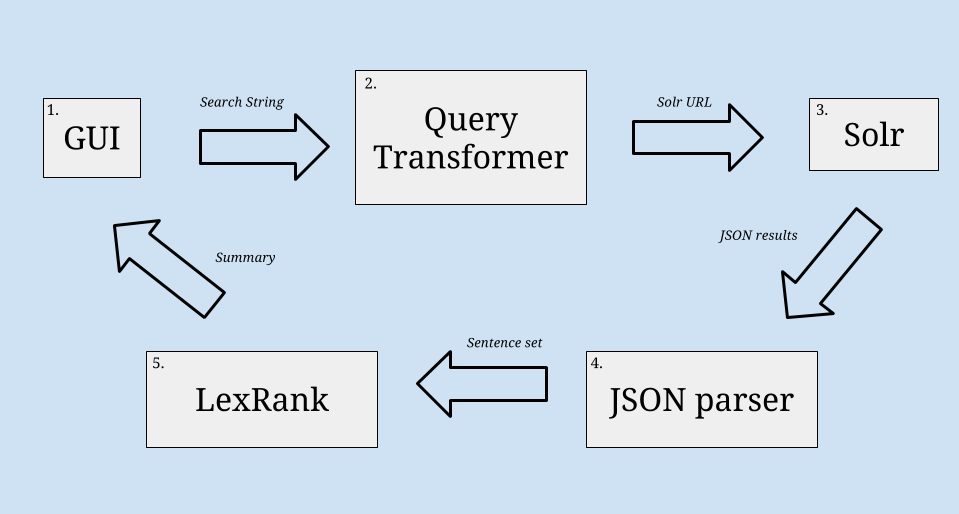
\includegraphics[width=1.0\textwidth]{IrProjectWorkFlowMedSiffror.png} 
   \caption{TODO: skriv bildtext}
   \label{fig:workflow}
\end{figure}


All sentences then continued to the LexRank implementation, which ranked the sentences according to relevance to the query. The highest ranked sentences from the LexRank algorithm were then sent to back to the GUI along with the titles of the Wikipedia article containing the sentence. 

\section{Resources}
The following subsections list the resources we used for our implementation.

\subsection{Wikipedia database}
Due to the massive size difference between english Wikipedia and its corresponding swedish set, we decided to use swedish Wikipedia as our source of data. Wikipedia provides their data for download in the format of XML (Extensible Markup Language). This is the only way to get all of Wikipedias articles, as Wikipedia does not want anyone to crawl their website in order to minimize traffic load. By using the database Apache Solr, it was then possible to import the XML-data and save the articles in a searchable format. As Wikipedia contains a lot of unwanted articles, such as redirects, portals, templates and categories; a regular expression pattern was used to skip those documents. \cite{wikidb}

\subsection{Apache Solr}
Solr is an open source search platform with features such as full-text search which is very scalable. It is written in Java and runs as a standalone server. It comes with a REST-api (Representational state transfer) where you can search by doing simple GET-requests. JSON was used as the result format for our searches, which was then parsed and used in our other algorithms. \cite{solr}

When doing full-text searches in all of the Wikipedia articles, Solr use by default a tf-idf scoring method with some modifications for ranking the articles. They have made what they call a Lucene's Practical Scoring Function, which it is based on the Vector Space Model (VSM). It uses td-idf scores in combination with document boosts (which is predefined scores of documents that should be ranked higher) and query boosts (some words in queries can be given higher priority). \cite{lucene}

\subsection{JavaFX}
JavaFX is a GUI library for Java and a software platform for creating and delivering rich internet applications (RIAs). We used it to create a desktop application from which a wikipedia search could be done. \cite{JavaFX}

\subsection{JSON-simple}
JSON-simple is a simple Java toolkit for encoding or decoding JSON text. We used it in order to decode the result from a Apache Solr query. \cite{JSONsimple}